\documentclass[a4paper,10pt]{article}
\usepackage[utf8]{inputenc}
\usepackage{polski}
\usepackage[polish]{babel}
\usepackage{graphicx}
\usepackage{amsmath}

% Title Page
\title{Projekt z eksploracji danych}
\author{Filip Chudy, Marcin Grzywaczewski}


\begin{document}
\maketitle

\begin{abstract}

\end{abstract}
\section{Opis danych i badanego zagadnienia}
\subsection{Dane}
W projekcie wykorzystany został Million Songs Dataset (Last.fm). 
Składa się on z informacji na temat miliona piosenek.
Każda piosenka reprezentowana jest jako JSON z następującymi elementami:
\begin{itemize}
 \item track\_id -- string, unikalny identyfikator piosenki
 \item similars -- lista par (track\_id, float) określająca podobieństwa między piosenkami wraz z ich ważnością (0-1)
 \item tags -- lista par (string, float) określająca tagi przypisane utworowi wraz z ich ważnością (0-100)
 \item artist -- string, nazwa artysty
 \item title -- string, tytuł piosenki
 \item timestamp -- string, czas zebrania danych
\end{itemize}

Z naszego punktu widzenia pole \textbf{timestamp} jest nieistotne.
Pola \textbf{artist} i \textbf{title} służą jedynie do prezentacji wyników.
Liczba utworów podobnych i podanych tagów jest zmienna, w szczególności mogą się zdarzyć takie utwory, które nie mają podanych tagów.
Liczba piosenek podanych w similars nie jest zbyt duża, co obrazuje histogram.
% TODO histogram

\subsection{Cel}
Celem projektu jest stworzenie systemu rekomendującego działającego na powyższych danych.
Zadanie jest trudne ze względu na rzadkość i niekompletność macierzy tagów i podobieństwa.

\section{Użyte metody}
\subsection{Wstęp}
Dane są rzadkie, więc wektoryzacja piosenek na podstawie tagów nie wchodziła w grę. 
Struktura \textbf{similars} przywodzi na myśl graf, dzięki czemu można uzupełnić macierz podobieństwa choćby za pomocą obliczenia przechodniego domknięcia.
Ponieważ w grafach naturalną miarą jest odległość, przeszliśmy z opisu opartego na podobieństwach na odległości według wzoru
\begin{equation}
 distance(x, y) = \frac{1}{similarity(x, y)}
\end{equation}

Metody wyznaczania przechodniego domknięcia grafu mają złożoność sześcienną względem liczby wierzchołków w grafie, 
więc aby którąś zastosować, należy zmniejszyć graf.

Pomysł na redukcję grafu wywodzi się z grupowania hierarchicznego.
Gęste skupiska punktów można reprezentować przy pomocy pojedynczych superwierzchołków, w których rozwiązywany będzie podobny problem dla tego skupiska.
Na tak wyznaczonych grafach hierarchicznych można już wyznaczyć przechodnie domknięcia.

\subsection{Algorytm hierarchiczny}
Algorytm kompresujący graf jest bardzo podobny w działaniu do algorytmów grupowania hierarchicznego.
Dane będą reprezentowane przez graf. Jego wierzchołki odpowiadają piosenkom lub ich zbiorom, a krawędzie -- odległościom między nimi.
W wierzchołkach grafu będzie przechowywana mniejsza wersja rozwiązywanego problemu.

Graf $G_1 = (V_1, E_1)$ jest przodkiem grafu $G_2 = (V_2, E_2)$, jeżeli istnieje taka krawędź $e(v_i, v_j) \in E_1$, że $V_1 \setminus \{v_i, v_j\} \subseteq V_2$, 
$V_2 \setminus V_1 = \{v_k\}$ i $inner\_vertices(v_k) = inner\_vertices(v_i) \cup inner\_vertices(v_j)$.\linebreak
Dodatkowo $(\forall w \in \{v: e(v_i, v) \in E_1 \vee e(v_j, v) \in E_1\})~e(v_k, w) \in E_2 \wedge |e(v_k, w)| = \min \{|e(u, w)| : u \in \{v_i, v_j\}\}$.
$G_2$ nazywamy potomkiem grafu $G_1$, jeśli $G_1$ jest przodkiem $G_2$.

Innymi słowy dla każdej krawędzi $e$ w grafie $G_1$ istnieje potomek $G_2$ grafu $G_1$ powstały przez scalenie wierzchołków łączonych przez $e$.
Oczywiście każda krawędź w grafie jednoznacznie wyznacza odpowiadającego jej potomka.

Każdemu grafowi przypisujemy koszt według pewnej funkcji błędu $F$.
W każdej iteracji wybieramy pewnego potomka $G_2$ grafu $G_1$ pod warunkiem, że $F(G_2) < F(G_1)$.
Ponieważ wyznaczanie wartości funkcji $F$ dla każdego potomka grafu $G_1$ byłoby kosztowne obliczeniowo, zastosowaliśmy wybór heurystyczny.

Wybieramy wierzchołek grafu o najmniejszym $inner\_vertices$.
Spośród krawędzi incydentnych do tego wierzchołka wybieramy najkrótszą taką krawędź $e(v_i, v_j)$, 
że graf $G_{ij}$ powstały przez scalenie $v_i$ i $v_j$ ma niższą funkcję błędu niż jego przodek.
Jeśli żadna z krawędzi incydentnych do wierzchołka nie zmniejsza funkcji kosztu, wybieramy kolejny wierzchołek według liczności $inner\_vertices$.

Wybór kończymy, jeśli każdy potomek grafu ma nie mniejszy koszt niż jego przodek lub przekroczymy minimalną wielkość grafu (parametr algorytmu).

\subsection{Funkcja kosztu}
Funkcja kosztu składa się z trzech czynników: WCD (rozmiary wewnętrzne superwierzchołków), 
SVP (penalizacja superwierzchołków jednoelementowych), BCD (odległości między superwierzchołkami).

\begin{equation}
 WCD(G) = \sum_{c \in C} \max_{e \in E(graph(c)} |e|
\end{equation}
\begin{equation}
 SVP(G) = |\{c \in C : size(c) = 1\}| \times \max_{e \in E(C)} |e|
\end{equation}
\begin{equation}
 BCD(G) = \sum_{c_1 \in C} \sum_{c_2 \in C} |e(c_1, c_2)|
\end{equation}

Sama funkcja kosztu jest iloczynem tych trzech czynników: 
\begin{equation}
F(G) = (WCD(G) + SVP(G)) \times BCD(G)
\end{equation}.


Obliczanie takiej funkcji jest kosztowne, jednak jeśli znamy wartości wszystkich czynników składających się na funkcję kosztu przodka, 
możemy na ich podstawie efektywnie wyznaczyć czynniki dla potomka.

Niech $G_2$ będzie potomkiem $G_1$ łączącym $c_i, c_j \in G_1$ w $c_k \in G_2$. Można zauważyć, że:
\begin{equation}
\begin{split}
 \Delta WCD(G_2) = WCD(G_2) - WCD(G_1)\\
 = \sum_{c \in C(G_2)} \max_{e \in E(graph(c))} |e| - \sum_{c \in C(G_1)} \max_{e \in E(graph(c))} |e|\\
 = \max_{e \in E(graph(v_k))} |e| - \max_{e \in E(graph(v_i))} |e| - \max_{e \in E(graph(v_j))} |e|
 \end{split}
\end{equation}

\begin{equation}
\begin{split}
 \Delta SVP(G_2) = SVP(G_2) - SVP(G_1)\\
 = |\{c \in \{v_i, v_j\} : size(c) = 1\}| \times \max_{e \in E(G)} |e|
 \end{split}
\end{equation}

\begin{equation}
\begin{split}
 \Delta BCD(G_2) = BCD(G_2) - BCD(G_1)\\
 = \sum_{c_1 \in C_2} \sum_{c_2 \in C_2} |e(c_1, c_2)| - \sum_{c_1 \in C_1} \sum_{c_2 \in C_1} |e(c_1, c_2)|\\
 = \sum_{c \in C_2} |e(v_k, c)| - \sum_{c \in C_1} |e(v_i, c)| - \sum_{c \in C_1} |e(v_j, c)| + |e(v_i, v_j)|
 \end{split}
\end{equation}

Dzięki temu obliczanie funkcji kosztu dla kolejnych potomków grafu jest znacznie szybsze.

\subsection{Ogląd globalny}
Początkowy graf dzielimy na spójne składowe algorytmem BFS. W każdej spójnej składowej wywołujemy opisany powyżej algorytm hierarchiczny.
Grafy na różnych poziomach hierarchii są na tyle małe, żeby dopełnić je do kliki za pomocą algorytmu Floyda-Warshalla.
Na tak dopełnionych grafach uruchomiony zostanie system rekomendujący.

\subsection{System rekomendujący}
System rekomendujący jako argument przyjmie piosenki \textbf{polubione} przez użytkownika.
System odnajduje zadane piosenki w grafie i zapisuje sobie ich sąsiadów. 
Jeśli sąsiadem jest superwierzchołek, do listy sąsiedztwa zostaje dodana cała jego zawartość (z odległością równą odległości między superwierzchołkami).
Mamy więc listę par piosenka-odległość (piosenka może na liście występować wielokrotnie, o tym za chwilę).
Na podstawie takiej listy zbudujemy dla każdej piosenki występującej na liście wartość liczbową mówiącą, jak dobrze nadaje się ona do rekomendacji.
Niech $distances_{s}$ oznacza [multi]zbiór odległości dla piosenki $s$.
\begin{equation}
 weight(s) = \sum_{d in distances(s)} d^{-1}
\end{equation}
W ten sposób dla każdej piosenki wyznaczamy odpowiadającą jej wartość liczbową. 
Rekomendacji dokonujemy losując bez zwracania odpowiednio wiele piosenek z zadanego przez $weight$ rozkładu dyskretnego z wagami.

\section{Implementacja}

Implementacja została podzielona na dwie części:
\begin{itemize}
 \item część przygotowania danych -- na tym etapie następuje normalizacja danych, 
	utworzenie lasu z podanych wierzchołków, zastosowanie algorytmu hierarchicznego oraz eksport powstałego wyniku do plików;
 \item część rekomendacji -- na tym etapie korzystamy z danych powstałych podczas poprzedniej fazy, 
	aby dla zadanego przez użytkownika zbioru utworów otrzymanym wynikiem były utwory zarekomendowane przez system.
\end{itemize}

Wyzwaniem okazała się złożoność pamięciowa. 
Istotnie trudnym problemem implementacyjnym okazało się opracowanie efektywnej procedury łączenia dwóch podgrafów w jeden -- 
jest to istotą naszego algorytmu hierarchicznego.

\subsection{Założenia na temat danych}

Przy analizie danych niezbędne okazały się następujące założenia na ich temat:
\begin{itemize}
 \item relacja podobieństwa danych powinna być symetryczna, więc dane zostały odpowiednio zmodyfikowane, aby założenie to spełnić,
 \item jeżeli podobieństwo utworu $A$ z $B$ wynosi $x$, podobieństwo utworu $B$ z $A$ również powinno wynosić $x$,
 \item grafy należące do lasu będące izolowanym wierzchołkiem nie niosą istotnej informacji dla systemu rekomendującego -- zostały one odrzucone,
 \item jeżeli w grafie istnieje krawędź $\left(v, w\right)$ to $v$ oraz $w$ istnieje w zbiorze danych.
\end{itemize}

Aby spełnić te założenia w implementacji uwzględniono odpowiednie procedury modyfikujące wejściowy zbiór danych.

\subsection{Poprawa symetryczności miary podobieństwa w zbiorze danych}

W celu poprawienia krawędzi zastosowano procedurę działającą w następujący sposób:
\begin{itemize}
 \item dla każdego wierzchołka $v$ występującego w grafie znajdujemy wszystkie krawędzie $\left(v, w\right)$,
 \item dla każdej krawędzi $\left(v, w\right)$ sprawdzamy jej miarę podobieństwa $p_{vw}$; jeżeli nie istnieje w grafie krawędź $\left(w, v\right)$, tworzymy ją nadając jej miarę podobieństwa $p_{vw}$,
 \item jeżeli krawędź $\left(w, v\right)$ istnieje, sprawdzamy jej miarę podobieństwa $p_{wv}$; ustalamy miarę podobieństwa obu krawędzi $\left(v, w\right)$ oraz $\left(w, v\right)$ na $p_{m}$, gdzie $p_{m}$ jest zdefiniowane jako $\max\{p_{vw}, p_{wv}\}$,
\end{itemize}

Powyższa procedura jest zaimplementowana jako \texttt{fix\_similarity\_symmetry} w module \texttt{load\_data} implementacji. Jej złożoność obliczeniowa to $\mathcal{O}\left(\left|V\right| + \left|E\right|\right)$. Jej wynikiem jest zbiór danych, który spełnia pierwsze i drugie założenie na temat danych.

\subsection{Usunięcie wierzchołków izolowanych krawędzi zewnętrznych zbioru danych} 

Po przeprowadzeniu procedury poprawy symetryczności krawędzi wierzchołki i krawędzie "nieprawidłowe" zostają usunięte z grafu. Za nieprawidłowe wierzchołki uważamy wierzchołki izolowane (tj. grafy w powstałym lesie zawierające dokładnie jeden wierzchołek). Za nieprawidłowe krawędzie uważamy krawędzie, których końce nie zawierają się w zbiorze danych.

Sposób działania procedury podobny do działania procedury poprawy symetryczności. Przechodzimy wszystkie wierzchołki $v$ występujące w grafie. Jeżeli liczba krawędzi wychodzących z tego wierzchołka to $0$, usuwamy taki wierzchołek. W przeciwnym wypadku przeglądamy wszystkie krawędzie $\left(v, w\right)$. Jeżeli wierzchołek $w$ nie istnieje w grafie, krawędź ta zostaje usunięta.

Odpowiadanie na pytanie "zawierania wierzchołka" jest zrealizowane w czasie stałym (struktura słownika). Całkowita złożoność procedury to $\mathcal{O}\left(\left|V\right| + \left|E\right|\right)$. Wynikiem działania procedury jest zbiór danych spełniający trzecie i czwarte założenie dotyczące danych.

Procedura jest zaimplementowana jako $\texttt{purge\_invalid\_vertices}$ w module $\texttt{load\_data}$.

\subsection{Poprawa złożoności pamięciowej: obcięcie danych}

W celu zaoszczędzenia pamięci wczytany zbiór danych został pozbawiony struktury $\texttt{tags}$ zawierającej tagi utworów. Identyfikatory utworów, będące łańcuchami znaków, zostały odwzorowane na zbiór $\{0, 1, \dots , n\}$. Wygenerowana mapa oraz mapa odwrotna tego odwzorowania jest zapisywana jako plik.

Oba te kroki są częścią procedury $\texttt{load\_data}$ w module $\texttt{load\_data}$.

\subsection{Algorytm wyznaczania lasu ze zbioru danych}

W celu wyznaczenia lasu ze zbioru danych zastosowany został klasyczny algorytm wyznaczania spójnych składowych. Wybranym sposobem przeglądania grafu został algorytm BFS. Całkowita złożoność wyznaczania obliczeniowa lasu to $\mathcal{O}\left(\left|V\right| + \left|E\right|\right)$. Jako wejście procedura akceptuje zbiór danych w postaci słownika odwzorowującego identyfikatory utworów w postaci liczb na obcięte dane zgodne z formatem plików oryginalnego zbioru danych. Wynikiem jest kolekcja obiektów typu $\texttt{Graph}$ realizujących logikę redukowania grafów i wyznaczania macierzy odległości.

Algorytm ten został zrealizowany jako obiekt $\texttt{Forest}$. Dostarczona została też procedura generująca reprezentację plikową już policzonego i zredukowanego lasu.

\subsection{Reprezentacja grafu}

Reprezentacja grafu musiała spełniać następujące warunki: w sposób efektywny obliczeniowo obsługiwać operacje wymagane przez algorytm redukcji, będąc jednocześnie odpowiednio wydajną pamięciowo. \textbf{Każdy wierzchołek w grafie jest podgrafem.}

Ostatecznym rozwiązaniem okazała się następująca implementacja:
\begin{itemize}
 \item w celu szybkiego dostępu do podgrafów grafu utrzymujemy słownik \texttt{subgraphs} będący odwzorowaniem identyfikatorów grafu (liczby $\{-1, -2, ..., -n\}$) na obiekty podgrafów,
 \item w celu szybkiego przeglądania krawędzi w grafie stosujemy strukturę \texttt{edges} będącą dwuwymiarowym słownikiem odwzorowującym parę identyfikatorów grafów $\left(v, w\right)$ na posortowaną rosnąco względem odległości listę krotek w postaci $\left(a, b, p\right)$ gdzie $a$ i $b$ to krawędź pomiędzy rzeczywistymi wierzchołkami, a $p$ to miara odległości (odwrotność miary podobieństwa). Z racji dwuwymiarowości możemy szybko odpowiadać na pytania typu \textit{wszystkie krawędzie incydentne z $v$} kosztem dwukrotnego zwiększenia złożoności pamięciowej dla kluczy,
 \item w celu wydajnego przeprowadzania redukcji utrzymujemy posortowany zbiór identyfikatorów podgrafów, zrealizowany jako drzewo czerwono-czarne; kluczem sortowania jest wielkość grafu -- preferujemy łączyć mniejsze grafy w większe.
\end{itemize}

\subsection{Redukcja grafu}

W celu redukowania grafu implementujemy algorytm opisany w poprzedniej sekcji raportu. Procedury \texttt{loss\_after\_merge} oraz \texttt{loss} są implementacjami odpowiednio: wartości funkcji błędu i wartości funkcji błędu po połączeniu pewnych podgrafów $v$ i $w$.

W procedurze $\texttt{reduce}$ realizujemy następujący algorytm.
\begin{itemize}
 \item dopóki znajdujemy wierzchołek $v$ mogący poprawić graf i liczba wierzchołków grafu jest większa niż pewna stała $M$:
  \begin{itemize}
    \item przeglądamy posortowaną rosnąco względem liczby krawędzi w podgrafie listę wierzchołków $v$:
    \begin{itemize}
    \item przeglądamy listę krawędzi $\left(v, w\right)$. Obliczamy funkcję błędu i funkcję błędu po scaleniu wierzchołków $v$ i $w$,
    \item jeżeli scalenie $\left(v, w\right)$ zmniejsza funkcję błędu, scalamy te wierzchołki w jeden podgraf. Oznaczamy iterację jako "udaną",
    \item jeżeli nie znajdujemy żadnej pary $\left(v, w\right)$ polepszającej funkcję błędu, przerywamy iterację.
    \end{itemize}
  \end{itemize}
\end{itemize}




\subsection{Łączenie podgrafów}

Łączenie podgrafów $(v, w)$ polega na stworzeniu nowego wierzchołka $G$ będącego nowym podgrafem aktualnie przetwarzanego grafu. Do tego podgrafu przenoszone są:
\begin{itemize}
 \item wszystkie wierzchołki należące do $v$ i $w$,
 \item wszystkie krawędzie od $v$ do $w$ (mamy tu na myśli listę połączeń realnych wierzchołków z wagami),
 \item wszystkie krawędzie wewnętrzne w $v$ i w $w$.
\end{itemize}

Poza tym należy przeprowadzić następujące kroki na poziomie aktualnie przetwarzanego grafu:

\begin{itemize}
 \item usunięcie wierzchołków $v$ i $w$,
 \item usunięcie krawędzi incydentnych z $v$ i $w$ (łączymy je z nowym grafem $G$),
 \item usunięcie krawędzi pomiędzy $v$ i $w$,
 \item przekierowanie wszystkich krawędzi $\left(v, x\right)$ i $\left(w, y\right)$ na krawędzie w postaci $\left(G, x\right)$, $\left(G, y\right)$, uwzględniając krawędzie odwrotne.
\end{itemize}

W celu łączenia dwóch posortowanych list będących wartością dwuwymiarowego słownika \texttt{edges} wprowadzona została metoda \texttt{merge\_sorted\_lists}. Operację łączenia podgrafów realizuje metoda \texttt{merge\_subgraphs} obiektu \texttt{Graph}.

\subsection{Obliczanie macierzy odległości}

Efektem redukcji grafu jest struktura, której liczba wierzchołków na pojedynczym poziomie jest odpowiednio zredukowana. Dzięki temu możemy policzyć macierz odległości. Macierz odległości liczona jest klasycznym algorytmem Floyda-Warshalla, działającym w czasie sześciennym od liczby wierzchołków w grafie.

Procedura ta jest zaimplementowana w obiekcie \texttt{Graph} jako \texttt{distance\_matrix}.

\subsection{Optymalizacja pamięciowa: Usuwanie nadmiarowych krawędzi}

Po zredukowaniu grafu przechwytywanie listy krawędzi z rzeczywistych wierzchołków i ich wag przestaje być potrzebne. Procedura \texttt{simplify\_edges} redukuje listę do jedynego interesującego nas w przypadku macierzy odległości elementu - krotki z najmniejszą odległością.

\subsection{Format wyjściowy}

Wyjściowym formatem dla grafów jest plik posiadający wewnątrz siebie listę identyfikatorów wierzchołków oraz macierz odległości między nimi. Procedura generowania tych plików (rekurencyjna) jest zrealizowana w obiekcie \texttt{Graph} jako \texttt{pickle\_graph}.

\subsection{System rekomendujący}
System rekomendujący realizowany jest przez klasę \texttt{Recommender}. Korzysta ona z wcześniej wyliczonych grafów leniwie odczytując je z dysku.
Do samej rekomendacji służy metoda \texttt{recommend}.
Przyjmuje ona listę utworów polubionych przez użytkownika i liczbę piosenek, którą system powinien dostarczyć.
Dla każdego polubionego utworu (i grafów leżących wyżej w hierarchii, które go zawierają) wyznaczamy listę kandydatów do rekomendacji i ich wagi.
Następnie losujemy bez zwracania potrzebną liczbę elementów.


\section{Wyniki}

Przedstawione tutaj wyniki są wytworzone poprzez analizę mniejszego zbioru danych (\textit{subset}) zawierającego około 9500 utworów muzycznych.
Niestety nie ma matematycznej miary poprawności rekomendacji. Niemniej jednak po ręcznym przeanalizowaniu otrzymanych wyników uznajemy efekty za zadowalające. System rekomenduje inne utwory tego samego artysty oraz artystów tworzących swoje albumy w podobnych czasach i stylach muzycznych. Nie jest to wystarczające do upewnienia się co do jakości systemu. Stąd też zostało zastosowane inne rozwiązanie.

\subsection{Przykłady}
Prezentujemy kilka przykładów symulowanych przez losowanie danych wejściowych i powiązanych z nimi rekomendacji:

Zapytany o piosenkę Scott Wesley Brown  --  All Rise system podał:
\begin{itemize}
 \item Mötley Crüe  --  Merry-Go-Round
 \item Ricky Martin  --  She's All I Ever Had
 \item Erja Lyytinen  --  Soul Of A Man
 \item Santana  --  Rock Me
 \item Scott Wesley Brown  --  I Stand Here Forgiven
\end{itemize}

Zapytany o piosenkę Jimmy Page  --  Liquid Mercury system podał:
\begin{itemize}
 \item Incubus  --  Just a Phase
 \item Beastie Boys  --  Flute Loop (2009 Digital Remaster)
 \item Yami Bolo  --  The Wonders
 \item The Police  --  Voices Inside My Head
 \item Otis Taylor  --  Round and Round
\end{itemize}

\subsection{Analiza jakości rekomendacji}

Z racji braku danych na temat wkładu użytkowników (odsłuchań i polubień) utworów klasyczne metody sprawdzania systemu rekomendacji nie mogły zostać tutaj użyte. Jedyne dostępne nam dane pozwalające ocenić rozwiązanie to tagi utworów. Przypomnijmy - tagi prezentowane są w postaci listy krotek $\left(n, p\right)$ gdzie $n$ jest etykietą danego tagu, a $p$ - wyrażoną od $1$ do $100$ "pewnością" należenia danego utworu do podanego tagu. Nasze rozwiązanie problemu walidacji rekomendacji oparliśmy na następującym pomyśle:

\begin{itemize}
 \item wytwarzamy \textit{sztucznego użytkownika} według następującej procedury: losujemy pewien utwór ze zbioru danych, nazwijmy go $T$. W kolejnym kroku algorytmu prosimy o 5 rekomendacji dla utworu $T$, po czym otrzymane rekomendacje dodajemy do zbioru 'wejściowego' dla kolejnych prób rekomendacji. W przypadku, gdy system nie potrafi zarekomendować pięciu utworów dla danego $T$, losujemy kolejny utwór, tworząc zbiór $\{T, T2\}$ i ponawiamy próbę. Proces kończymy, gdy uda nam się zgromadzić 100 utworów.
 \item dla wytworzonego \textit{sztucznego użytkownika} reprezentowanego przez zbiór utworów $\{ t_{1}, t_{2}, \dots, t_{100} \}$ prosimy o kolejne 5 rekomendowanych utworów.
 \item Przez $C$ oznaczmy zbiór utworów stanowiący sztucznego użytkownika. Przez $R$ zaś - zbiór utworów zarekomendowanych przez tego użytkownika. Na zbiorach $C$ i $R$ wykonujemy procedurę \textit{gromadzenia tagów}.
\end{itemize}

\subsection{Gromadzenie tagów}

Dla danego zbioru $X$ utworów muzycznych gromadzenie tagów wytwarza pewien agregat $aggregated\_tags\left(X\right)$ zdefiniowany następująco:

\begin{itemize}
 \item jeżeli dla każdego $t \in X$ jest oznaczone pewnym tagiem o etykiecie $e$, agregat zawiera tag o tej etykiecie.
 \item dla każdego tagu o etykiecie $e$ w agregacie, jego "pewność" wyrażona jest jako $\frac{\sum^{n}_{i=1} p_{i}}{N}$ gdzie $n$ to liczba utworów oznaczonych tagiem z etykietą $e$, $N$ - liczba utworów muzycznych o niepustej liście tagów, zaś $p_{i}$ jest "pewnością" tagu o etykiecie $e$ dla $i$-tego utworu oznaczonego tagiem z etykietą $e$.
\end{itemize}

Tak przygotowany agregat tagów jest wykorzystywany w dalszej analizie poprawności systemu.

\subsection{Funkcja błędu}

Naszym założeniem przy ocenie systemu rekomendującego jest to, że dla dowolnego utworu muzycznego $t$ jego rekomendacja $t\prime$ jest oznaczana przez podobne tagi. Aby "mierzyć" to podobieństwo wykorzystaliśmy dwie funkcje błędu:

\begin{itemize}
 \item Funkcja błędu oparta o odległość Manhattan - naturalna i prosta do analizy miara błędu.
 \item Funkcja błędu średniokwadratowego - w celu porównania z poprzednią funkcją błędu. Nie bardzo wiadomo co oznaczają wartości tej funkcji.
\end{itemize}

W przypadku tych błędów "odległością" mierzoną przez funkcję błędu jest różnica "pewności" dla tagów z agregatu tagów dla \textit{sztucznego użytkownika} i kolejnych pięciu rekomendacji. Przy obliczaniu funkcji błędu nie bierzemy pod uwagę tagów o bardzo małej pewności - zakładamy, że są zaburzeniami i odrzucamy je. W przypadku, gdy agregat $X$ jest oznaczany tagiem o etykiecie $e$, a drugi agregat nie - zakładamy że "pewność" dla drugiego agregatu tagu o etykiecie $e$ wynosi $0$.

\subsection{Wyniki testowania}

W celu przeprowadzenia analizy wylosowaliśmy 100 par sztucznych użytkowników i ich kolejnych pięciu rekomendacji. Dla każdej z tych par wyliczyliśmy funkcję błędu MDE (\textit{Manhattan Distance Error}) oraz MSE (\textit{Mean Squared Error}). Poniżej przedstawiamy histogram wartości obu funkcji błędów, podzielonych przez liczbę tagów w agregatach:

\begin{figure}[h]
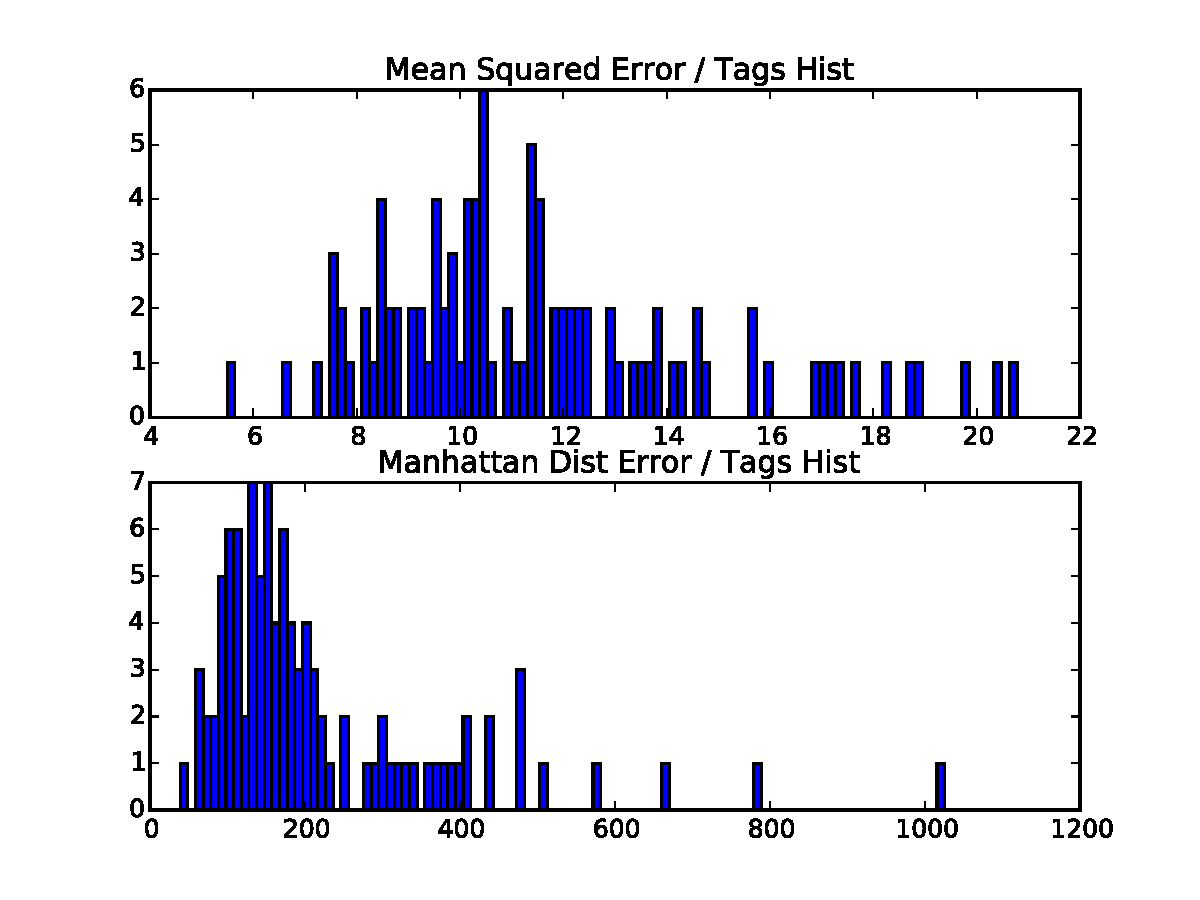
\includegraphics[width=\textwidth,height=\textheight,keepaspectratio]{mde_mse_hist_subset.pdf}
\caption{Histogram zastosowanych funkcji błędu}
\end{figure}

Jak można zauważyć, wartości funkcji MDE wskazują na wysoką skuteczność systemu - wartości oscylują w okolicach wartości $10$. Przy zakresie od zera do stu "pewności" tagów, których może być wiele jest to wartość pożądana - oznacza to, że wśród WSZYSTKICH istotnych tagów łączna różnica ich "pewności" oscyluje w granicach tej wartości. Oczywiście wszystko zależy od liczności agregatów tagów. W przypadku sztucznych użytkowników uśredniona liczność odpowiadającego mu agregatu oscylowała dookoła wartości $2000$. W przypadku agregatu kolejnych rekomendacji było to $160$. Liczby te uwzględniają tagi nieistotne, wycięte podczas liczenia funkcji błędu - niemniej jednak pozwalają mieć ogólny wgląd w to, jak liczne są to zbiory.

Warto wspomnieć o pomysłach, które okazały się nieudane - pierwszym naszym pomysłem na funkcję błędu była f. błędu bazująca na indeksie Giniego. Z racji jej własności (etykiety tagów byłyby nierozróżnialne) i trudności w zdefiniowaniu prawdopodobieństwa należenia do analizowanego przez indeks zbioru odrzuciliśmy ten pomysł jako nietrafiony.

\section{Wnioski końcowe, podsumowanie, perspektywy rozwoju}

Pomimo posiadania wiedzy na temat lokalnego podobieństwa utworów muzycznych, utworzenie miar przechodniego (tudzież "globalnego") podobieństwa pewnych utworów muzycznych okazało się wyzwaniem. System rekomendujący przedstawiony w tym projekcie jest przykładem systemu opartego na idei \textit{content-based-filtering}. Wiedza, którą generuje z informacji zadanych w zbiorze danych, jest wiedzą wynikającą wyłącznie z własności przedmiotów rekomendowanych (w tym wypadku -- utworów muzycznych). Z racji operowania pojęciem macierzy podobieństwa (która jest obiektem pamięciowo rozległym) wymagane były skomplikowane operacje grupowania danych.

Wielkość opracowywanego zbioru danych sugerowałaby użycie podejść typu \textit{collaborative filtering}. Niestety nie posiadaliśmy danych o użytkownikach i ich ocenach/preferencjach dotyczących utworów -- stąd też rowiązanie jest oparte na potencjalnie "gorszej" idei. Niemniej jednak systemy tego typu sprawdzają się lepiej w przypadku, gdy zgromadzonych danych jest niewiele -- nie zależą też od ocen użytkowników.

Perspektywy rozwoju tego systemu leżą w ulepszeniu istniejącej implementacji (usprawnienie obliczeń, zmniejszenie zużycia pamięci) oraz implementacji nowych elementów mających wpływ na wyniki rekomendacji:

\begin{enumerate}
  \item Możliwe jest wprowadzenie wyborów użytkownika -- mógłby on oznaczać pewne utwory jako nielubiane. System rekomendacyjny karałby wtedy utwory znajdujące się w bezpośrednim otoczeniu (odległości) od takich utworów.
  \item Możliwa jest także dalsza regularyzacja funkcji błędu. Rozważanym przez nas pomysłem było m.in. wprowadzenie czynnika \textit{maksymalnej liczności wierzchołków grafu}. System rekomendacyjny karałby wtedy za podgrafy zawierające zbyt wiele elementów.
\end{enumerate}


\end{document}          
